\documentclass[a4paper,11pt,titlepage]{article}

\usepackage{latexsym}
\usepackage{graphicx}
\usepackage{float}
\usepackage{url}
\usepackage{unicode}
\usepackage[polish]{babel}
\usepackage{titlesec}
\usepackage{listings}
\usepackage{xcolor}
\usepackage{setspace}
\usepackage{subfig}
\usepackage{tabularx}
\usepackage{courier}
\DeclareUnicodeCharacter{200B}{{\hskip 0pt}}

\definecolor{codeblue}{rgb}{0,0,0.6}
\definecolor{codegray}{rgb}{0.5,0.5,0.5}
\definecolor{codepurple}{rgb}{0.58,0,0.82}
\definecolor{backcolour}{rgb}{0.96,0.96,0.96}

\lstdefinestyle{code}{
    backgroundcolor=\color{backcolour},
    keywordstyle=\color{codeblue},
    numberstyle=\tiny\color{codegray},
    stringstyle=\color{codeblue},
    basicstyle=\ttfamily\footnotesize,
    breakatwhitespace=false,
    breaklines=true,
    captionpos=b,
    keepspaces=true,
    numbers=left,
    numbersep=3pt,
    showspaces=false,
    showstringspaces=false,
    showtabs=false,
    tabsize=1,
    basicstyle=\small
}

\lstset{style=code}

\newcommand{\sectionbreak}{\clearpage}
\author{Adam Talarczyk}
\title{Symulacje Monte Carlo}
\frenchspacing
\begin{document}
\begin{titlepage}
    \begin{center}

        \Huge
        \textbf{WYDZIAŁ NAUK ŚCISŁYCH I TECHNICZNYCH}
        
        
        \vspace{1.5cm}
	   Symulacje Komputerowe
        \LARGE
        
	\vspace{2cm}
	
	Sprawozdanie ``Symulacja zdarzeń dyskretnych''

	\vspace{1cm}
	Adam Talarczyk, Mateusz Wrzoł
	
	\vspace{5cm}
        \vfill

        \vspace{0.8cm}
	\Large
        Uniwersytet Śląski, Sosnowiec, 2021

    \end{center}
\end{titlepage}
\newpage

%\tableofcontents
% \newpage


\section{Zadanie 1}
Wykonać symulację bramek autostradowych uwzględniając następujące założenia:
\begin{itemize}
	\item Dostępne są cztery bramki. Na trzech bramkach kierowcy mogą płacić kartą i gotówką. Na jednej bramce kierowcy mogą płacić tylko kartą.
	\item Czas trwania obsługi na bramce w przypadku płatności gotówką jest opisany rozkładem normalnym o średniej M1 minuty i odchyleniu standardowym SD1 minuty.
	\item Czas trwania obsługi na bramce w przypadku płatności kartą jest opisany rozkładem normalnym o średniej M2 minuty i odchyleniu standardowym SD2 minuty.
	\item Odstęp czasu pomiędzy nadjeżdżającymi samochodami jest opisany rozkładem wykładniczym o parametrze lambda = L (wartość oczekiwana wynosi 1/L minuty, L odpowiada średniej liczbie pojazdów na minutę).
	\item Połowa kierowców zamierza dokonać płatności kartą a druga połowa gotówką. Nadjeżdżający kierowcy wybierają dostępną bramkę z najkrótszą kolejką. Płacący gotówką mają do wyboru 3 bramki. Płacący kartą wybierają spośród 4 bramek.
	Wartości parametrów
	\end{itemize}

\begin{figure}[H]
 \centering
 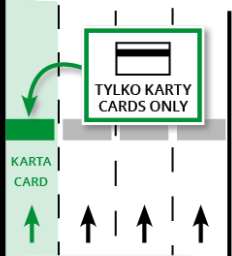
\includegraphics[width=0.35\columnwidth]{img/tresc.PNG}
 \caption{Wizualizacja}
 \label{fig:wykres1}
\end{figure}

Wartości parametrów SD1, SD2, M1 i M2 należy przyjąć według własnego uznania.

Wyznaczyć symulacyjnie zależność pomiędzy średnią liczbą pojazdów na minutę (L) i średnim czasem oczekiwania na przejazd przez bramki. Przedstawić tę zależność na wykresie.

W sprawozdaniu należy zamieścić treść zadania, kod źródłowy rozwiązania z opisem, wyniki symulacji i wykres.


\subsection{Rozwiązanie}
Zachowanie kierowców zostało zdefiniowane w osobnej, parametryzowanej funkcji. Każdemu kierowcy przypisać można alias słuzący do wyświetlania logów, dostępne bramki (parametr \verb|gates|) oraz czas przejazdu przez bramki wraz z odchyleniem standardowym. Na podstawie funkcji driver  (Listing \ref{listing-driver}) utworzono obiekty dla kierowców płacących gotówką i kartą oraz samą gotówką. W założeniach przyjęto, że dostępne bramki autostradowe oznaczane są jako \verb|gate1, gate2, gate3, gate4|. Kierowcy płacący tylko i wyłącznie gotówką mają do dyspozycji bramki \verb|gate2, gate3 oraz gate4|, ponieważ \verb|gate1| obsługuje tylko karty. Przy założeniu, że płatność kartą odbywa się szybciej, przyjęto parametr \verb|M1=3, SD1=2| dla płatności gotówką, oraz \verb|M2=2, SD1=1| dla płatności kartą.

Symulacja jest również sparametryzowaną funkcją (Listing \ref{listing-symulacja}), w której można ustawić parametr L (cars\_per\_minute), obiekty kierowców (cash/card\_drivers\_trajectory) oraz łączną liczbę kierowców. Symulacja wykonywana jest pętli, dla parametru L z przedziału od 1 do 10, przy założeniu 50 kierowców płacących kartą jak i 50 kierowców płacących gotówką. Dla każdego parametru L wyniki zostały powtórzone 10 razy a następnie uśrednione. Jak widać na listingu \ref{listing-symulacja}, definiowane są dostępne bramki oraz ilość kierowców wraz z ich typem (cash/card\_drivers\_trajectory). Wyniki, czyli średni czas oczekiwania do przejazdu oraz średni czas płacenia przy bramkach zostały wyeksportowane do arkusza kalkulacyjnego.

Na podstawie danych utworzony wykres (Rysunek \ref{fig:wykres}), który przedstawia czas oczekiwania na przejazd względem parametru L, przy łącznej ilości 100 kierowców. Uśrednione dane z 10 prób przedstawione są w tabeli \ref{tab:res}.

\begin{figure}[H]
 \centering
 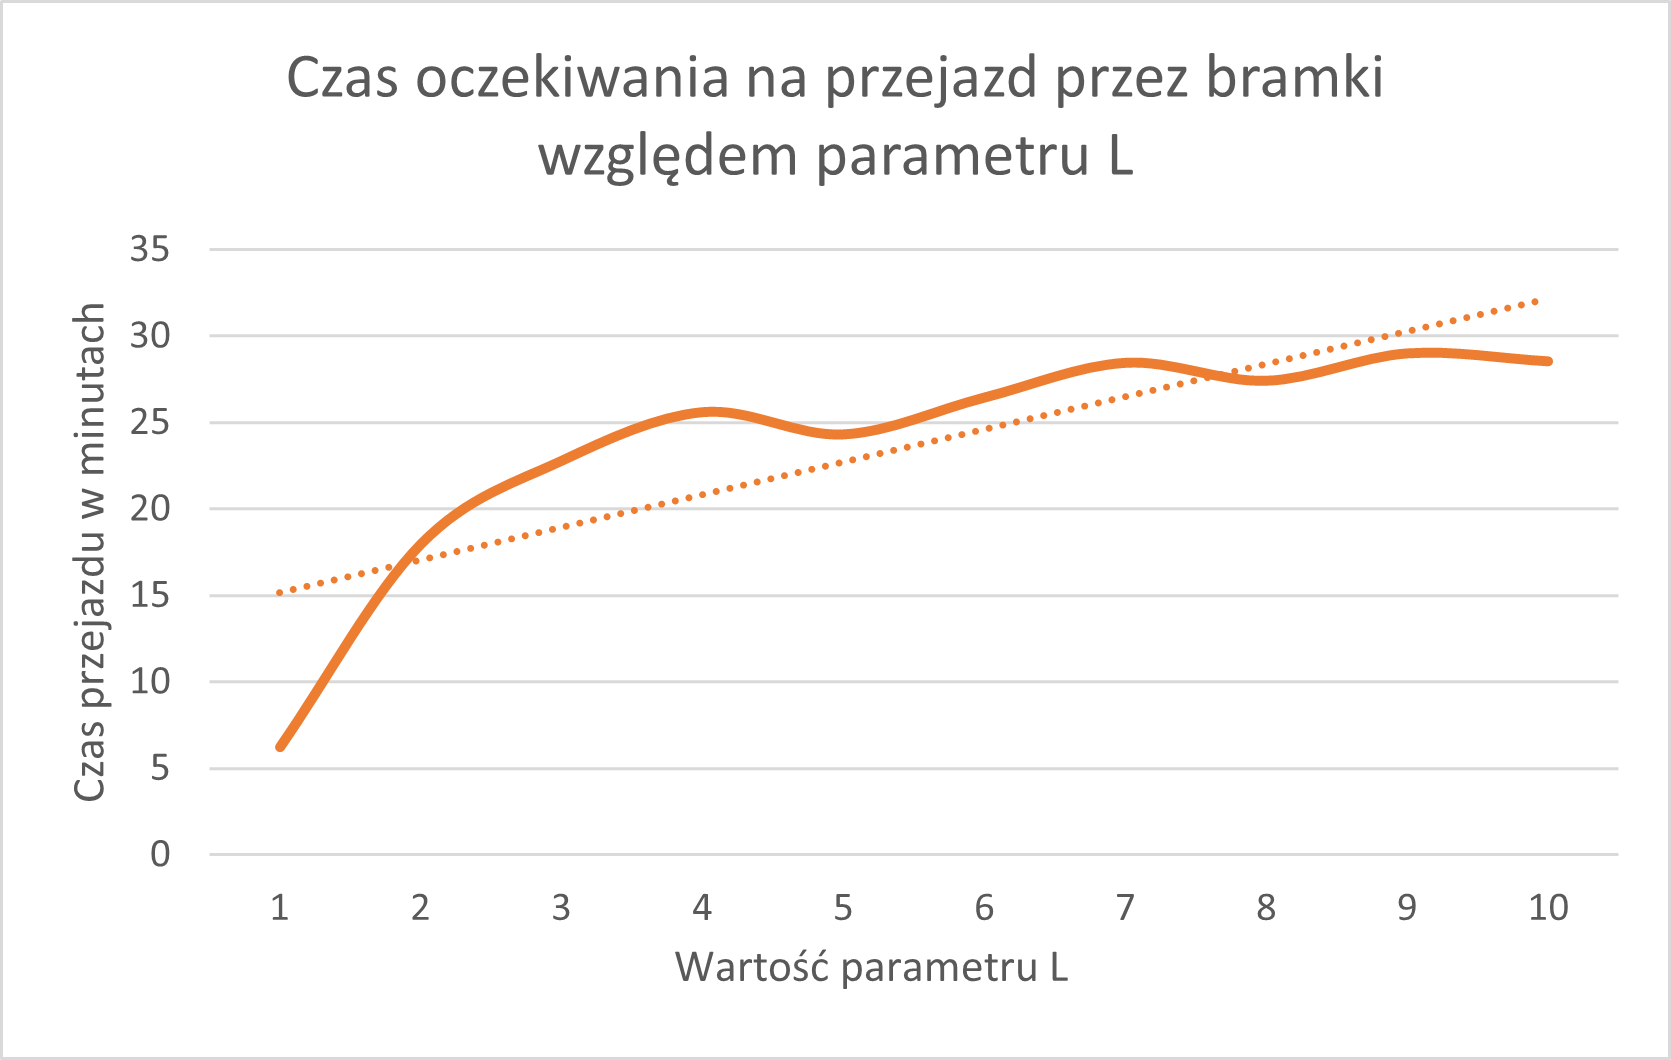
\includegraphics[width=1\columnwidth]{img/wykres3.PNG}
 \caption{Wykres przedstawiający czas oczekiwania na przejazd przez bramki względem parametru L przy 100 kierowcach}
 \label{fig:wykres}
\end{figure}

 \begin{table}[h!]
 \centering
 \begin{tabular}{ |c|c|c| } 
 \hline
 Parametr L & Średni czas przejazdu przez bramki \\
 \hline
1 &	6.229830525 \\
2 &	17.96801664 \\
3 &	22.78144309 \\
4 &	25.58758123 \\
5 &	24.29923589 \\
6 &	26.43225118 \\
7 &	28.43579926 \\
8 &	27.39886657 \\
9 &	28.97951878 \\
10 &	28.52141024 \\

 \hline
\end{tabular}
\caption{Tablica z wynikami uzyskanymi w symulacji}
\label{tab:res}
 \end{table}

Na podstawie powyższych danych i wykresu widać, że czas oczekiwania na przejazd przez bramki rośnie wraz z parametrem L.

\subsection{Kod źródłowy}

\lstinputlisting[language=R, caption=Funkcja związana z zachowaniem kierowcy, label={listing-driver}]{../simulation/driver.R}
\lstinputlisting[language=R, caption=Imlementacja symulacji, label={listing-symulacja}]{../simulation/simulate_gates.R}
\lstinputlisting[language=R, caption=Wywołanie symulacji kilkukrotnie dla różnych wartości i zapis danych do pliku, label={listing-main}]{../simulation/main.R}

\end{document}
